\documentclass[aspectratio=169,11pt]{beamer}

% ---------------------------------------------------------------------
% MedTrace Rubric-Aligned Review Presentation
% Compile on Overleaf with pdfLaTeX.
% ---------------------------------------------------------------------

\usetheme{Madrid}
\usecolortheme{default}
\usefonttheme{professionalfonts}

\usepackage[T1]{fontenc}
\usepackage[utf8]{inputenc}
\usepackage{lmodern}
\usepackage{booktabs}
\usepackage{array}
\usepackage{tabularx}
\usepackage{tikz}
\usepackage{xcolor}

\definecolor{Ink}{HTML}{23313A}
\definecolor{Blue}{HTML}{1E5F7A}
\definecolor{Teal}{HTML}{1E9A8A}
\definecolor{Coral}{HTML}{C95C55}
\definecolor{Sand}{HTML}{F4EEE6}
\definecolor{Soft}{HTML}{EAF5F3}
\definecolor{Gold}{HTML}{D99A23}
\definecolor{Slate}{HTML}{5D6A72}

\setbeamercolor{title}{fg=white}
\setbeamercolor{frametitle}{fg=Ink,bg=Sand}
\setbeamercolor{structure}{fg=Blue}
\setbeamercolor{block title}{fg=white,bg=Blue}
\setbeamercolor{block body}{fg=Ink,bg=Soft}
\setbeamercolor{alerted text}{fg=Coral}
\setbeamercolor{normal text}{fg=Ink}
\setbeamertemplate{navigation symbols}{}
\setbeamertemplate{footline}[frame number]
\setbeamersize{text margin left=7mm,text margin right=7mm}
\setlength{\tabcolsep}{4pt}
\renewcommand{\arraystretch}{1.14}

\newcommand{\pill}[2]{%
  \tikz[baseline=(X.base)]\node[rounded corners=6pt, fill=#1, inner xsep=7pt, inner ysep=3pt] (X) {\scriptsize\textbf{#2}};%
}

\newcommand{\scorebox}[2]{%
  \begin{minipage}{0.31\linewidth}
    \centering
    {\Large\textbf{#1}}\\[-1mm]
    {\scriptsize #2}
  \end{minipage}
}

\title[MedTrace]{MedTrace}
\subtitle{Endometriosis Longitudinal Intelligence Platform}
\author{50\% Implementation Review}
\institute{Final Year Project}
\date{\today}

\begin{document}

% ---------------------------------------------------------------------
\begin{frame}[plain]
  
\begin{tikzpicture}[remember picture,overlay]
    \fill[Blue] (current page.south west) rectangle (current page.north east);
    \fill[Teal,opacity=0.28] (current page.south west) .. controls +(3,2) and +(-2,-2) .. ([xshift=3cm]current page.north east) -- (current page.north east) -- (current page.south east) -- cycle;
    \fill[Coral,opacity=0.18] ([xshift=-1cm,yshift=-1cm]current page.north east) circle (2.5cm);
  \end{tikzpicture}
  \vspace{1.0cm}
  {\color{white}\Huge\textbf{MedTrace}}\\[2mm]
  {\color{white}\Large Endometriosis Longitudinal Intelligence Platform}\\[7mm]
  {\color{white}\large Rubric-aligned evidence of current implementation, technical correctness and interim results}\\[10mm]
  \pill{white}{Working 50\% Core Implementation}
  \hfill
  {\color{white}\small Final Year Project Review}
\end{frame}

% ---------------------------------------------------------------------
\begin{frame}{Review Criteria Mapping}
  \scriptsize
  \begin{tabularx}{\linewidth}{>{\bfseries}p{0.23\linewidth} X c}
    \toprule
    Criterion & What this presentation demonstrates & Marks \\
    \midrule
    Implementation & Working modules covering the core intelligence layer, UI screens, demo data, analytics and report generation. & 5 \\
    Technical Accuracy & Correct data model, statistical methods, evidence gates, deterministic engine and tested implementation practices. & 5 \\
    Results Obtained So Far & Interim metrics from synthetic evaluation, test results, validation tables and interpretation. & 5 \\
    \bottomrule
  \end{tabularx}

  \vspace{3mm}
  \begin{block}{Claim for this review}
    We have completed the central 50\% of the approved scope: the working longitudinal intelligence prototype. The remaining work is production completion: secure accounts, encrypted storage, backend synchronization, sharing workflow, mobile deployment and pilot validation.
  \end{block}
\end{frame}

% ---------------------------------------------------------------------
\begin{frame}{Project Objective}
  \begin{block}{Problem addressed}
    Endometriosis-related symptoms are longitudinal: they vary across days, menstrual cycles, medication use, treatment periods and healthcare events. During a short consultation, this history is difficult for the patient to reconstruct accurately.
  \end{block}

  \begin{block}{System objective}
    MedTrace builds a structured symptom history from low-burden daily entries, computes clinically meaningful longitudinal patterns, and produces a concise clinician-facing summary with traceable supporting evidence.
  \end{block}

  \begin{center}
    \pill{Teal!20}{Low-burden capture}
    \hspace{2mm}
    \pill{Gold!30}{Deterministic analysis}
    \hspace{2mm}
    \pill{Coral!20}{Evidence-backed brief}
  \end{center}
\end{frame}

% ---------------------------------------------------------------------
\begin{frame}{Approved Scope vs Current Progress}
  \scriptsize
  \begin{tabularx}{\linewidth}{>{\bfseries}p{0.25\linewidth} X X}
    \toprule
    Scope Area & Current Status & Evidence \\
    \midrule
    Patient symptom capture & Implemented as adaptive daily check-in & Today screen, symptom chips, impact and medication fields \\
    Structured longitudinal record & Implemented using typed TypeScript data model & PatientRecord, DayRecord, TreatmentEpisode, ClinicalEvent \\
    Cycle-aware analytics & Implemented & Cycle segmentation and phase alignment engine \\
    Pattern detection & Implemented & Pattern engine with findings and suppressed findings \\
    Clinician summary & Implemented & Brief screen with evidence drawer \\
    Validation & Implemented & Evaluation harness, metrics file, automated tests \\
    Production infrastructure & Planned next phase & Authentication, encrypted DB, backend, consent and sharing \\
    \bottomrule
  \end{tabularx}
\end{frame}

% ---------------------------------------------------------------------
\begin{frame}{Implementation: Executable Modules Completed}
  \begin{columns}[T]
    \column{0.5\linewidth}
      \begin{block}{Frontend modules}
        \begin{itemize}
          \item Today: daily adaptive check-in
          \item Patterns: heatmap and findings
          \item Timeline: symptoms, treatments and events
          \item Brief: clinician summary and evidence drawer
          \item Validation: engine metrics
          \item Method: design explanation
        \end{itemize}
      \end{block}
    \column{0.5\linewidth}
      \begin{block}{Engine modules}
        \begin{itemize}
          \item Cycle segmentation
          \item Feature extraction
          \item Statistical pattern detection
          \item Baseline change detection
          \item Brief generation
          \item Fidelity verification
          \item Synthetic evaluation harness
        \end{itemize}
      \end{block}
  \end{columns}
\end{frame}

% ---------------------------------------------------------------------
\begin{frame}{Implementation Architecture}
  \begin{center}
  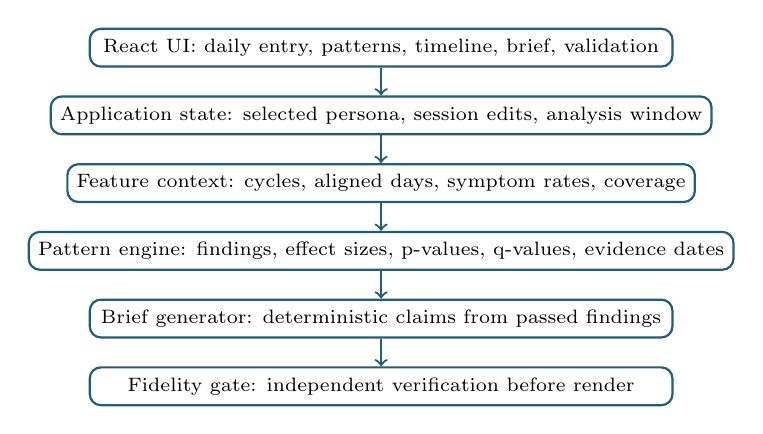
\begin{tikzpicture}[
    node distance=0.86cm,
    box/.style={rounded corners, draw=Blue, fill=white, thick, minimum width=7.4cm, minimum height=0.48cm, align=center, font=\scriptsize},
    arr/.style={->, thick, draw=Blue}
  ]
    \node[box] (a) {React UI: daily entry, patterns, timeline, brief, validation};
    \node[box, below of=a] (b) {Application state: selected persona, session edits, analysis window};
    \node[box, below of=b] (c) {Feature context: cycles, aligned days, symptom rates, coverage};
    \node[box, below of=c] (d) {Pattern engine: findings, effect sizes, p-values, q-values, evidence dates};
    \node[box, below of=d] (e) {Brief generator: deterministic claims from passed findings};
    \node[box, below of=e] (f) {Fidelity gate: independent verification before render};
    \draw[arr] (a) -- (b);
    \draw[arr] (b) -- (c);
    \draw[arr] (c) -- (d);
    \draw[arr] (d) -- (e);
    \draw[arr] (e) -- (f);
  \end{tikzpicture}
  \end{center}

  \vspace{1mm}
  \begin{block}{Attributable implementation evidence}
    These modules are present in the submitted codebase and execute through the Vite app, automated tests and evaluation script.
  \end{block}
\end{frame}

% ---------------------------------------------------------------------
\begin{frame}{Implementation: Demo Patients}
  \scriptsize
  \begin{tabularx}{\linewidth}{>{\bfseries}p{0.15\linewidth} p{0.22\linewidth} X}
    \toprule
    Persona & Scenario & What this demonstrates \\
    \midrule
    Maya & Suspected endometriosis & Clear perimenstrual pattern, bowel symptoms, functional burden and consultation timeline. \\
    Priya & Confirmed endometriosis, on treatment & Persistent non-cyclical pain and before/during treatment comparison. \\
    Aisha & Sparse logger & Evidence gate withholding findings when data coverage is insufficient. \\
    \bottomrule
  \end{tabularx}

  \vspace{2mm}
  \begin{block}{Why demo patients are useful}
    Each persona exercises a different behavior: detection, treatment comparison, and safe refusal when evidence is weak.
  \end{block}
\end{frame}

% ---------------------------------------------------------------------
\begin{frame}{Technical Accuracy: Literature and Survey Driven Choices}
  \begin{columns}[T]
    \column{0.5\linewidth}
      \begin{block}{From literature review}
        \begin{itemize}
          \item Capture pain, bowel, urinary, fatigue and impact domains
          \item Separate symptom severity from functional impact
          \item Use menstrual timing as clinical context
          \item Show data completeness and avoid missing-data assumptions
        \end{itemize}
      \end{block}
    \column{0.5\linewidth}
      \begin{block}{From survey/user needs}
        \begin{itemize}
          \item Keep daily logging short
          \item Support patient-specific symptom vocabulary
          \item Make sensitive areas optional
          \item Generate a useful consultation summary
        \end{itemize}
      \end{block}
  \end{columns}

  \vspace{4mm}
  \begin{center}
    \pill{Gold!30}{Design outcome: rich underlying model, minimal daily interaction}
  \end{center}
\end{frame}

% ---------------------------------------------------------------------
\begin{frame}{Technical Accuracy: Data Model}
  \small
  \begin{tabularx}{\linewidth}{>{\bfseries}p{0.22\linewidth} X}
    \toprule
    Model Layer & Implemented meaning \\
    \midrule
    Baseline profile & Age range, diagnosis status, symptom onset, prior labels, family history and cycle baseline. \\
    Daily records & Date, logged status, bleeding, impact, symptom states, medication and logging depth. \\
    Event records & Treatment episodes and healthcare events such as consultations, ultrasound and surgery. \\
    Derived layer & Cycle day, phase angle, rates, trends, coverage, findings, claims and evidence dates. \\
    \bottomrule
  \end{tabularx}

  \vspace{4mm}
  \begin{block}{Tri-state rule}
    Every symptom observation is treated as present, absent or unknown. A skipped or unasked symptom is unknown and excluded from denominators. This is technically important because missing data should not be counted as symptom-free.
  \end{block}
\end{frame}

% ---------------------------------------------------------------------
\begin{frame}{Technical Accuracy: Cycle-Aware Analysis}
  \begin{block}{Design choice}
    The engine does not assume a standard 28-day cycle. It segments cycles from recorded bleeding onsets and aligns symptoms relative to each observed cycle.
  \end{block}

  \begin{center}
  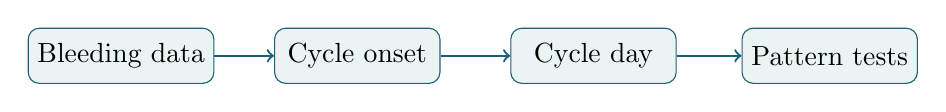
\begin{tikzpicture}
    \node[rounded corners, draw=Blue, fill=Soft, minimum width=2.1cm, minimum height=0.7cm] (a) at (0,0) {Bleeding data};
    \node[rounded corners, draw=Blue, fill=Soft, minimum width=2.1cm, minimum height=0.7cm] (b) at (3,0) {Cycle onset};
    \node[rounded corners, draw=Blue, fill=Soft, minimum width=2.1cm, minimum height=0.7cm] (c) at (6,0) {Cycle day};
    \node[rounded corners, draw=Blue, fill=Soft, minimum width=2.1cm, minimum height=0.7cm] (d) at (9,0) {Pattern tests};
    \draw[->, thick, Blue] (a) -- (b);
    \draw[->, thick, Blue] (b) -- (c);
    \draw[->, thick, Blue] (c) -- (d);
  \end{tikzpicture}
  \end{center}

  \begin{block}{Why this is correct for the domain}
    Endometriosis symptoms are often interpreted relative to menstruation. Using recorded cycles preserves individual variation and avoids forcing irregular cycles into an artificial average.
  \end{block}
\end{frame}

% ---------------------------------------------------------------------
\begin{frame}{Technical Accuracy: Statistical Methods}
  \scriptsize
  \begin{tabularx}{\linewidth}{>{\bfseries}p{0.25\linewidth} p{0.27\linewidth} X}
    \toprule
    Question & Implemented method & Reason \\
    \midrule
    Symptom near menstruation? & Fisher's exact test & Works with small counts common in few-cycle records. \\
    Where does it peak? & Rayleigh test on phase angles & Treats the cycle as circular rather than linear. \\
    Getting worse? & Mann--Kendall and Theil--Sen & Robust for short, ordinal longitudinal series. \\
    Symptoms together? & Cohen's kappa + permutation & Discounts chance overlap between common symptoms. \\
    Changed after treatment? & Exact Poisson rate comparison & Suitable for before/during event rates. \\
    Multiple tests? & Benjamini--Hochberg q-values & Controls false discoveries across pattern families. \\
    \bottomrule
  \end{tabularx}
\end{frame}

% ---------------------------------------------------------------------
\begin{frame}{Technical Accuracy: Evidence Gate}
  \begin{block}{Why an evidence gate is needed}
    A health summary should not present patterns that are based on very little data. Therefore, the engine computes possible findings but reports only those that pass data sufficiency and statistical criteria.
  \end{block}

  \begin{columns}[T]
    \column{0.5\linewidth}
      \begin{block}{Gate requirements}
        \begin{itemize}
          \item Minimum observation coverage
          \item Minimum complete cycles
          \item Minimum symptom occurrences
          \item Statistical significance after correction
        \end{itemize}
      \end{block}
    \column{0.5\linewidth}
      \begin{block}{User-visible behavior}
        \begin{itemize}
          \item Strong findings are shown
          \item Weak findings are withheld
          \item Withheld findings include reasons
          \item Absence of evidence is not hidden
        \end{itemize}
      \end{block}
  \end{columns}
\end{frame}

% ---------------------------------------------------------------------
\begin{frame}{Technical Accuracy: Brief Generation and Verification}
  \begin{block}{Implemented report strategy}
    The clinician brief is generated from typed findings. Sentences are template-based, and numeric values are filled from computed results rather than manually written.
  \end{block}

  \begin{block}{Fidelity checker}
    Before claims are displayed, key values are independently re-derived from raw day records. If a claim does not match the underlying record, it is removed from the displayed summary.
  \end{block}

  \begin{center}
    \pill{Teal!20}{Computed findings}
    \hspace{2mm}
    \pill{Gold!30}{Templated claims}
    \hspace{2mm}
    \pill{Coral!20}{Independent verification}
  \end{center}
\end{frame}

% ---------------------------------------------------------------------
\begin{frame}{Results: Automated Test Evidence}
  \begin{center}
    \scorebox{111}{automated tests}
    \scorebox{3}{engine test files}
    \scorebox{0}{manual statistics in report}
  \end{center}

  \vspace{3mm}
  \begin{block}{What the tests cover}
    \small
    \begin{itemize}
      \item Statistical reference values and helper functions
      \item Cycle segmentation and phase alignment
      \item Missing-data invariants
      \item Pattern-engine determinism
      \item Evidence-date attachment
      \item Diagnostic-language safety checks
      \item Brief fidelity and mutation rejection
    \end{itemize}
  \end{block}
\end{frame}

% ---------------------------------------------------------------------
\begin{frame}{Results: Cyclicity Detection Experiment}
  \scriptsize
  \begin{tabularx}{\linewidth}{>{\bfseries}p{0.32\linewidth} c c c c}
    \toprule
    Classifier & Precision & Recall & F1 & False Patterns \\
    \midrule
    MedTrace full engine & 0.977 & 0.649 & 0.780 & 2 \\
    Ratio rule baseline & 0.856 & 0.908 & 0.881 & 20 \\
    Missing-as-zero baseline & 0.850 & 0.908 & 0.878 & 21 \\
    \bottomrule
  \end{tabularx}

  \vspace{3mm}
  \begin{block}{Interpretation}
    The simple ratio rule finds more patterns but produces many more false patterns. MedTrace prioritizes precision because a clinician-facing summary should avoid presenting unsupported patterns as reliable.
  \end{block}
\end{frame}

% ---------------------------------------------------------------------
\begin{frame}{Results: Missing Data Robustness}
  \scriptsize
  \begin{tabularx}{\linewidth}{>{\bfseries}p{0.18\linewidth} c c c c}
    \toprule
    Scenario & Coverage & F1 gated & Precision gated & F1 ungated \\
    \midrule
    MCAR 10\% drop & 90\% & 0.85 & 0.95 & 0.85 \\
    MCAR 30\% drop & 71\% & 0.71 & 1.00 & 0.76 \\
    MCAR 40\% drop & 59\% & 0.10 & 1.00 & 0.67 \\
    MAR 30\% drop & 80\% & 0.70 & 1.00 & 0.70 \\
    MAR 50\% drop & 69\% & 0.57 & 0.95 & 0.60 \\
    \bottomrule
  \end{tabularx}

  \vspace{2mm}
  \begin{block}{Interpretation}
    As coverage falls, the evidence gate becomes conservative. This is intentional: the system prefers to withhold weak findings rather than overstate unreliable patterns.
  \end{block}
\end{frame}

% ---------------------------------------------------------------------
\begin{frame}{Results: Brief Fidelity}
  \scriptsize
  \begin{tabularx}{\linewidth}{>{\bfseries}p{0.42\linewidth} c X}
    \toprule
    Metric & Result & Meaning \\
    \midrule
    Claims verified & 226 / 226 & Untampered generated claims passed verification. \\
    Injected mutations caught & 194 / 194 & Corrupted numeric claims were rejected. \\
    Verified key coverage & 59.5\% & A substantial share of displayed numbers were independently re-derived. \\
    \bottomrule
  \end{tabularx}

  \vspace{3mm}
  \begin{block}{Interpretation}
    This supports the core promise that the brief is evidence-traceable. The mutation test is especially important because it shows the checker can catch altered values rather than only approving correct claims.
  \end{block}
\end{frame}

% ---------------------------------------------------------------------
\begin{frame}{Results: Logging Burden}
  \scriptsize
  \begin{tabularx}{\linewidth}{>{\bfseries}p{0.36\linewidth} c c c}
    \toprule
    Comparator & Fields per day & Reduction & Estimated time \\
    \midrule
    Adaptive planner & 6.8 & -- & 24 sec \\
    Fixed own-vocabulary questionnaire & 9.0 & 24.1\% & 32 sec \\
    Fixed full-vocabulary questionnaire & 37.0 & 81.5\% & 130 sec \\
    \bottomrule
  \end{tabularx}

  \vspace{3mm}
  \begin{block}{Interpretation}
    This result supports the main product design decision: the system can maintain a rich health model while showing only a few relevant fields during daily logging.
  \end{block}
\end{frame}

% ---------------------------------------------------------------------
\begin{frame}{Results: Runtime Feasibility}
  \begin{block}{Evaluation included latency measurement}
    The evaluation harness measures the time taken for feature extraction, pattern detection, brief generation and fidelity verification on generated longitudinal records.
  \end{block}

  \begin{block}{Technical interpretation}
    The current prototype runs the full analysis synchronously in the browser for demo-scale records. This supports feasibility for an interactive prototype, and heavier future workloads can be moved to backend jobs if needed.
  \end{block}

  \begin{center}
    \pill{Teal!20}{Feature extraction}
    \hspace{2mm}
    \pill{Gold!30}{Pattern engine}
    \hspace{2mm}
    \pill{Coral!20}{Brief + verification}
  \end{center}
\end{frame}

% ---------------------------------------------------------------------
\begin{frame}{Current Deliverables}
  \begin{columns}[T]
    \column{0.5\linewidth}
      \begin{block}{Executable deliverables}
        \begin{itemize}
          \item Web app prototype
          \item Demo patient workflows
          \item Pattern engine
          \item Clinician brief screen
          \item Automated tests
          \item Evaluation script
        \end{itemize}
      \end{block}
    \column{0.5\linewidth}
      \begin{block}{Documentation deliverables}
        \begin{itemize}
          \item Product requirements document
          \item Build log
          \item Competitive/methodology analysis
          \item PDF target design
          \item Validation metrics
          \item Presentation deck
        \end{itemize}
      \end{block}
  \end{columns}
\end{frame}

% ---------------------------------------------------------------------
\begin{frame}{Work Remaining for 100\% Completion}
  \scriptsize
  \begin{tabularx}{\linewidth}{>{\bfseries}p{0.28\linewidth} X}
    \toprule
    Remaining Area & Planned implementation \\
    \midrule
    Secure onboarding & User registration, baseline profile collection and module preferences. \\
    Data security & Encrypted local storage, backend database, authentication and access control. \\
    Offline-first mobile app & React Native application with reliable local entry and background sync. \\
    Patient-defined symptoms & Custom symptom creation, patient terminology and standardized mapping. \\
    AI-assisted intake & Voice/text entry converted into structured candidate records after confirmation. \\
    Sharing workflow & Patient preview, consent, report export, share grants and audit trail. \\
    Pilot evaluation & Feedback from users and clinicians to refine the report and workflow. \\
    \bottomrule
  \end{tabularx}
\end{frame}

% ---------------------------------------------------------------------
\begin{frame}{Completion Roadmap}
  \begin{center}
  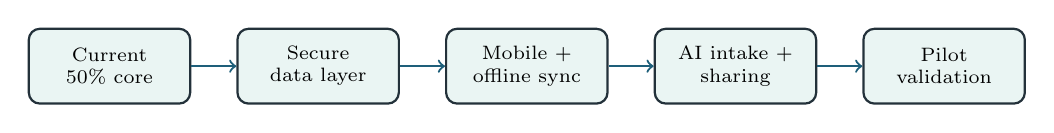
\begin{tikzpicture}[
    stage/.style={rounded corners, draw=Ink, fill=Soft, thick, minimum width=2.05cm, minimum height=0.95cm, align=center, font=\scriptsize},
    arr/.style={->, thick, draw=Blue}
  ]
    \node[stage] (s1) at (0,0) {Current\\50\% core};
    \node[stage] (s2) at (2.65,0) {Secure\\data layer};
    \node[stage] (s3) at (5.3,0) {Mobile +\\offline sync};
    \node[stage] (s4) at (7.95,0) {AI intake +\\sharing};
    \node[stage] (s5) at (10.6,0) {Pilot\\validation};
    \draw[arr] (s1) -- (s2);
    \draw[arr] (s2) -- (s3);
    \draw[arr] (s3) -- (s4);
    \draw[arr] (s4) -- (s5);
  \end{tikzpicture}
  \end{center}

  \vspace{4mm}
  \begin{block}{Strategy}
    The core analytical solution is already implemented. The next phase focuses on making it secure, mobile, shareable and suitable for supervised real-world evaluation.
  \end{block}
\end{frame}

% ---------------------------------------------------------------------
\begin{frame}{Conclusion}
  \small
  \begin{block}{Implementation evidence}
    The submitted project demonstrates working modules across data capture, longitudinal record assembly, cycle-aware analytics, pattern detection, clinician summary generation and validation.
  \end{block}

  \begin{block}{Technical accuracy evidence}
    The design uses correct missing-data handling, cycle alignment, statistical tests, multiplicity correction, evidence gating and independent verification.
  \end{block}

  \begin{block}{Results evidence}
    Current results include automated tests, detection metrics, robustness analysis, fidelity mutation testing, logging-burden comparison and validation outputs.
  \end{block}

  \centering
  \textbf{MedTrace converts low-burden symptom tracking into evidence-traceable clinical context.}
\end{frame}

% ---------------------------------------------------------------------
\begin{frame}[plain]
  \begin{tikzpicture}[remember picture,overlay]
    \fill[Ink] (current page.south west) rectangle (current page.north east);
    \fill[Teal,opacity=0.22] (current page.south west) circle (4.1cm);
    \fill[Coral,opacity=0.18] (current page.north east) circle (3.1cm);
  \end{tikzpicture}
  \vspace{2.0cm}
  \centering
  {\color{white}\Huge\textbf{Thank You}}\\[5mm]
  {\color{white}\Large Questions and Demonstration}\\[12mm]
  \pill{white}{MedTrace 50\% Implementation Review}
\end{frame}

\end{document}
